\documentclass[11pt,a4paper]{article}
%\usepackage{fontspec, xunicode, xltxtra}  
%\setmainfont{Hiragino Sans GB}  
%\usepackage{xeCJK}
%\setCJKmainfont[BoldFont=STZhongsong, ItalicFont=STKaiti]{STSong}
%\setCJKsansfont[BoldFont=STHeiti]{STXihei}
%\setCJKmonofont{STFangsong}

%使用Xelatex编译

% 设置页面
%==================================================
\linespread{2} %行距
% \usepackage[top=1in,bottom=1in,left=1.25in,right=1.25in]{geometry}
% \headsep=2cm
% \textwidth=16cm \textheight=24.2cm
%==================================================

% 其它需要使用的宏包
%==================================================
\usepackage[colorlinks,linkcolor=blue,anchorcolor=red,citecolor=green,urlcolor=blue]{hyperref} 
\usepackage{tabularx}
\usepackage{authblk}         % 作者信息
\usepackage{algorithm}     % 算法排版
\usepackage{amsmath}     % 数学符号与公式
\usepackage{amsfonts}     % 数学符号与字体
\usepackage{amssymb}
\usepackage[framemethod=TikZ]{mdframed}

\usepackage{graphicx} 
\usepackage{graphics}
\usepackage{color}
\usepackage{xcolor}
\usepackage{tcolorbox}
\usepackage{lipsum}
\usepackage{empheq}

\usepackage{fancyhdr}       % 设置页眉页脚
\usepackage{fancyvrb}       % 抄录环境
\usepackage{float}              % 管理浮动体
\usepackage{geometry}     % 定制页面格式
\usepackage{hyperref}       % 为PDF文档创建超链接
\usepackage{lineno}          % 生成行号
\usepackage{listings}        % 插入程序源代码
\usepackage{multicol}       % 多栏排版
%\usepackage{natbib}         % 管理文献引用
\usepackage{rotating}       % 旋转文字,图形,表格
\usepackage{subfigure}    % 排版子图形
\usepackage{titlesec}       % 改变章节标题格式
\usepackage{moresize}   % 更多字体大小
\usepackage{anysize}
\usepackage{indentfirst}  % 首段缩进
\usepackage{booktabs}   % 使用\multicolumn
\usepackage{multirow}    % 使用\multirow

\usepackage{wrapfig}

\usepackage{titlesec}     % 改变标题样式
\usepackage{enumitem}

\renewcommand{\vec}[1]{\boldsymbol{#1}}
\newcommand{\me}{\mathrm{e}}
\newcommand{\mi}{\mathrm{i}}
\newcommand{\dif}{\mathrm{d}}
\newcommand{\tabincell}[2]{\begin{tabular}{@{}#1@{}}#2\end{tabular}}

\def\kpc{{\rm kpc}}
\def\km{{\rm km}}
\def\cm{{\rm cm}}
\def\TeV{{\rm TeV}}
\def\GeV{{\rm GeV}}
\def\MeV{{\rm MeV}}
\def\GV{{\rm GV}}
\def\MV{{\rm MV}}
\def\yr{{\rm yr}}
\def\s{{\rm s}}
\def\ns{{\rm ns}}
\def\GHz{{\rm GHz}}
\def\muGs{{\rm \mu Gs}}
\def\arcsec{{\rm arcsec}}
\def\K{{\rm K}}
\def\microK{\mu{\rm K}}
\def\sr{{\rm sr}}
\newcolumntype{p}{D{,}{\pm}{-1}}

\renewcommand{\figurename}{Fig.}
\renewcommand{\tablename}{Tab.}

\renewcommand{\arraystretch}{1.5}

\setlength{\parindent}{0pt}  %取消每段开头的空格


\newcounter{theo}[section]\setcounter{theo}{0}
\renewcommand{\thetheo}{\arabic{section}.\arabic{theo}}
\newenvironment{theo}[2][]{%
\refstepcounter{theo}%
\ifstrempty{#1}%
{\mdfsetup{%
frametitle={%
\tikz[baseline=(current bounding box.east),outer sep=0pt]
\node[anchor=east,rectangle,fill=blue!20]
{\strut Theorem~\thetheo};}}
}%
{\mdfsetup{%
frametitle={%
\tikz[baseline=(current bounding box.east),outer sep=0pt]
\node[anchor=east,rectangle,fill=blue!20]
{\strut Theorem~\thetheo:~#1};}}%
}%
\mdfsetup{innertopmargin=10pt,linecolor=blue!20,%
linewidth=2pt,topline=true,%
frametitleaboveskip=\dimexpr-\ht\strutbox\relax
}
\begin{mdframed}[]\relax%
\label{#2}}{\end{mdframed}}

\newcommand*\widefbox[1]{\fbox{\hspace{2em}#1\hspace{2em}}}


\title{First Order Ordinary Differential Equation}
\author{}
\date{\today}
\begin{document}

\maketitle

\section{The Existence and Uniqueness of Solutions}
\cite{george1991differential, simmons2016differential} 

\section{First Order Equations}
\subsection{Homogeneous Equations}
\cite{george1991differential, simmons2016differential} 
\begin{equation*}
\frac{\dif y}{\dif x} = f(x, y)
\end{equation*}
No formulas exist for obtaining its solution in all cases. 

When the variables are separable:
\begin{eqnarray*}
\frac{\dif y}{\dif x} = g(x)h(y) \\
\frac{\dif y}{h(y)} = g(x) \dif x \\
\int \frac{\dif y}{h(y)} = \int g(x) \dif x +c
\end{eqnarray*}

A function $f(x,y)$ is called \textcolor{red}{homogeneous of degree $n$} if
\begin{equation*}
f(tx, ty) = t^n f(x, y)
\end{equation*}
for all suitably restricted $x$, $y$, and $t$.

The differential equation
\begin{equation*}
M(x, y) \dif x +N(x, y)\dif y =0
\end{equation*}
is said to be \textcolor{red}{homogeneous} if $M$ and $N$ are homogeneous functions of the same degree. This equation can then be written in the form
\begin{equation*}
\frac{\dif y}{\dif x} = f(x, y)
\end{equation*}
where $f(x, y) = -\dfrac{M(x, y)}{N(x, y)}$ is clearly homogeneous of degree $0$. It can always be changed into an equation with separable variables by means of the substitution $z = y/x$, regardless of the form of the function $f(x,y)$.
\begin{eqnarray*}
f(x,y) = f(1, y/x) = f(1, z)
\end{eqnarray*}
Since $y=zx$, 
\begin{equation*}
\frac{\dif y}{\dif x} = z +x\frac{\dif z}{\dif x} ~,
\end{equation*}
then
\begin{eqnarray*}
z +x\frac{\dif z}{\dif x} = f(1, z) \\
\frac{\dif z}{f(1, z) -z} = \frac{\dif x}{x}
\end{eqnarray*}

\subsection{Exact Equations}
For the differential equation
\begin{equation}
M(x, y) \dif x +N(x, y)\dif y =0 ~,
\label{exact}
\end{equation}
if there happens to exist a function $f(x,y)$,
\begin{eqnarray}
\frac{\partial f}{\partial x} = M ~, ~~{\rm and } ~~ \frac{\partial f}{\partial y} = N ~,
\label{exact_dr}
\end{eqnarray}
\begin{equation*}
\frac{\partial f}{\partial x} \dif x +\frac{\partial f}{\partial y} \dif y = 0 ~, ~~{\rm or } ~~ \dif f = 0
\end{equation*}
and its general solution is
\begin{equation*}
f(x, y) = c ~.
\end{equation*}
The expression $M\dif x + N\dif y$ is said to be an \textcolor{red}{exact differential}, and equ. (\ref{exact}) is called an \textcolor{red}{exact differential equation}.

Suppose that equ. (\ref{exact}) is exact, so that there exists a function $f$ satisfying equations (\ref{exact_dr}). From
\begin{equation*}
\frac{\partial^2 f}{\partial y \partial x} = \frac{\partial^2 f}{\partial x \partial y} ~,
\end{equation*}
\begin{equation}
\frac{\partial M}{\partial y} = \frac{\partial N}{\partial x} ~,
\label{exact_con}
\end{equation}
so (\ref{exact_con}) is a necessary condition for the exactness of (\ref{exact}).


\subsection{Integrating Factors}
If
\begin{equation}
M(x, y) \dif x +N(x, y)\dif y =0 ~,
\end{equation}
is not exact, find a function $\mu(x,y)$ to make
\begin{equation*}
\mu(M\dif x + N\dif y) = 0
\end{equation*}
an exact differential.


\subsection{Linear Equations}
\textcolor{red}{Linear equation}: the derivative of highest order is a linear function of the lower order derivatives. The general first order linear equation is
\begin{equation*}
\frac{\dif y}{\dif x} = p(x) y +q(x) ~,
\end{equation*}
and the general second order linear equation is
\begin{equation*}
\frac{\dif^2 y}{\dif x^2} = p(x) \frac{\dif y}{\dif x} +q(x) y +r(x)  ~.
\end{equation*}

The standard form of the general first order linear equation is
\begin{equation}
\frac{\dif y}{\dif x} +P(x) y = Q(x) ~.
\end{equation}
Since
\begin{equation*}
\frac{\dif }{\dif x} \left(e^{\int P \dif x} \right) = e^{\int P \dif x} \frac{\dif y}{\dif x} +y Pe^{\int P \dif x} = e^{\int P \dif x} \left( \frac{\dif y}{\dif x} +Py\right) ~,
\end{equation*}
\begin{equation}
\frac{\dif }{\dif x} \left(e^{\int P \dif x} y \right) = Q e^{\int P \dif x} ~.
\end{equation}
\begin{align}
\nonumber e^{\int P \dif x} y &= \int Q e^{\int P \dif x}  \dif x +c ~, \\
y &= e^{-\int P \dif x} \left( \int Q e^{\int P \dif x}  \dif x +c \right)
\end{align}

\subsection{Reduction of Order}



































\section{Systems of First Order Equations}
































\subsection{Nonlinear Systems. Volterra's Prey-Predator Equations}
\cite{george1991differential, simmons2016differential} Imagine an island inhabited by foxes and rabbits. The foxes eat rabbits, and the rabbits eat clover. We assume that there is so much clover that the rabbits always have an ample supply of food. When the rabbits are abundant, then the foxes flourish and their population grows. When the foxes become too numerous and eat too many rabbits, they enter a period of famine and their population begins to decline. As the foxes decrease, the rabbits become relatively safe and their population starts to increase again. This triggers a new increase in the fox population, and as time goes on we see an endlessly repeated cycle of interrelated increases and decreases in the populations of the two species. 

If $x$ is the number of rabbits at time $t$, then we should have
\begin{equation}
\dfrac{\dif x}{\dif t} = a x ~,  ~~~ a > 0 ~,
\end{equation}
as a consequence of the unlimited supply of clover, if the number $y$ of foxes is zero. It is natural to assume that the number of encounters per unit time between rabbits and foxes is jointly proportional to $x$ and $y$. If further assuming that a certain proportion of these encounters result in a rabbit being eaten, then 
\begin{equation}
\dfrac{\dif x}{\dif t} = a x - b xy ~,  ~~~ a~ \text{and}~ b > 0 ~,
\end{equation}
In the same way
\begin{equation}
\dfrac{\dif y}{\dif t} = - cy + d xy ~,  ~~~ c~ \text{and}~ d > 0 ~,
\end{equation}
for in the absence of rabbits the foxes die out, and their increase depends on the number of their encounters with rabbits. The following nonlinear system describes the interaction of these two species:
\begin{equation}
\left\{
\begin{aligned}
\dfrac{\dif x}{\dif t} &= x(a  - b y) ~, \\
\dfrac{\dif y}{\dif t} &= - y(c - d x) ~. 
\end{aligned}
\right.
\label{eq:Volterra}
\end{equation}
Equations (\ref{eq:Volterra}) are called Volterra's prey-predator equations. On eliminating $t$ in (\ref{eq:Volterra}) by division, and separating the variables,
\begin{equation}
\dfrac{(a-by)\dif y}{y} = -\dfrac{(c-dx)\dif x}{x} ~.
\end{equation}
\begin{align}
\nonumber  a \log y - by &= -c \log x +d x + \log K ~, \\
y^a {\rm e}^{-by} &= K x^{-c} {\rm e}^{dx} ~,
\label{eq:Volterra_sol}
\end{align}
where the constant $K$ is given by
\begin{equation}
K = x_0^{c} y_0^a {\rm e}^{-dx_0 -by_0}
\end{equation}
in terms of the initial values of $x$ and $y$.

Equate the left and right sides of (\ref{eq:Volterra_sol}) to new variables $z$ and $w$, and then plot the graphs $C_1$ and $C_2$ of the functions
\begin{equation}
\left\{
\begin{aligned}
z &= y^a {\rm e}^{-by} ~, \\
w &= K x^{-c} {\rm e}^{dx} ~,
\end{aligned}
\right.
\label{eq:z_w}
\end{equation}
as shown in Fig. \ref{fig:Volterra}. Since $z=w$, we are confined in the third quadrant to the dotted line $L$. To the maximum value of $z$ given by the point $A$ on $C_1$, there corresponds one $y$ and - via $M$ on $L$ and the corresponding points $A^\prime$ and  $A^{\prime \prime}$ on $C_2$ - two x's, and these determine the bounds between which $x$ may vary. Similarly, the minimum value of $w$ given by $B$ on $C_2$ leads to $N$ on $L$ and hence to $B^\prime$ and $B^{\prime \prime}$ on $C_1$ and these points determine the bounds for $y$. In this way we find the points $P_1$, $P_2$ and $Q_1$, $Q_2$ on the desired curve $C_3$. Additional points are easily found by starting on $L$ at a point $R$ anywhere between $M$ and $N$ and projecting up to $C_1$ and over to $C_3$, and then over to $C_2$ and up to $C_3$. Changing the value of $K$ raises or lowers the point $B$, and this expands or contracts the curve $C_3$. When $K$ is given various values, we obtain a family of ovals about the point $S$, which is all there is of $C_3$ when the minimum value of w equals the maximum value of $z$.

As $t$ increases, the corresponding point $(x, y)$ on $C_3$ moves around the curve in a counterclockwise direction. Begin by noting that equations (\ref{eq:Volterra}) give the horizontal and vertical components of the velocity of this point. A simple calculation based on formulas (\ref{eq:z_w}) shows that the point $S$ has coordinates $x=c/d$, $y=a/b$. When $x < c/d$, it follows from the second equation of (\ref{eq:Volterra}) that $\dif y/\dif t$ is negative, so our point on $C_3$ moves down as it traverses the arc $Q_2 P_1 Q_1$. Similarly, it moves up along the arc $Q_1 P_2 Q_2$.


Use the fox-rabbit problem to illustrate the important method of linearization. First, we observe that if the rabbit and fox populations are

%**********************************Figure 1***************************************
\begin{figure}
\centering
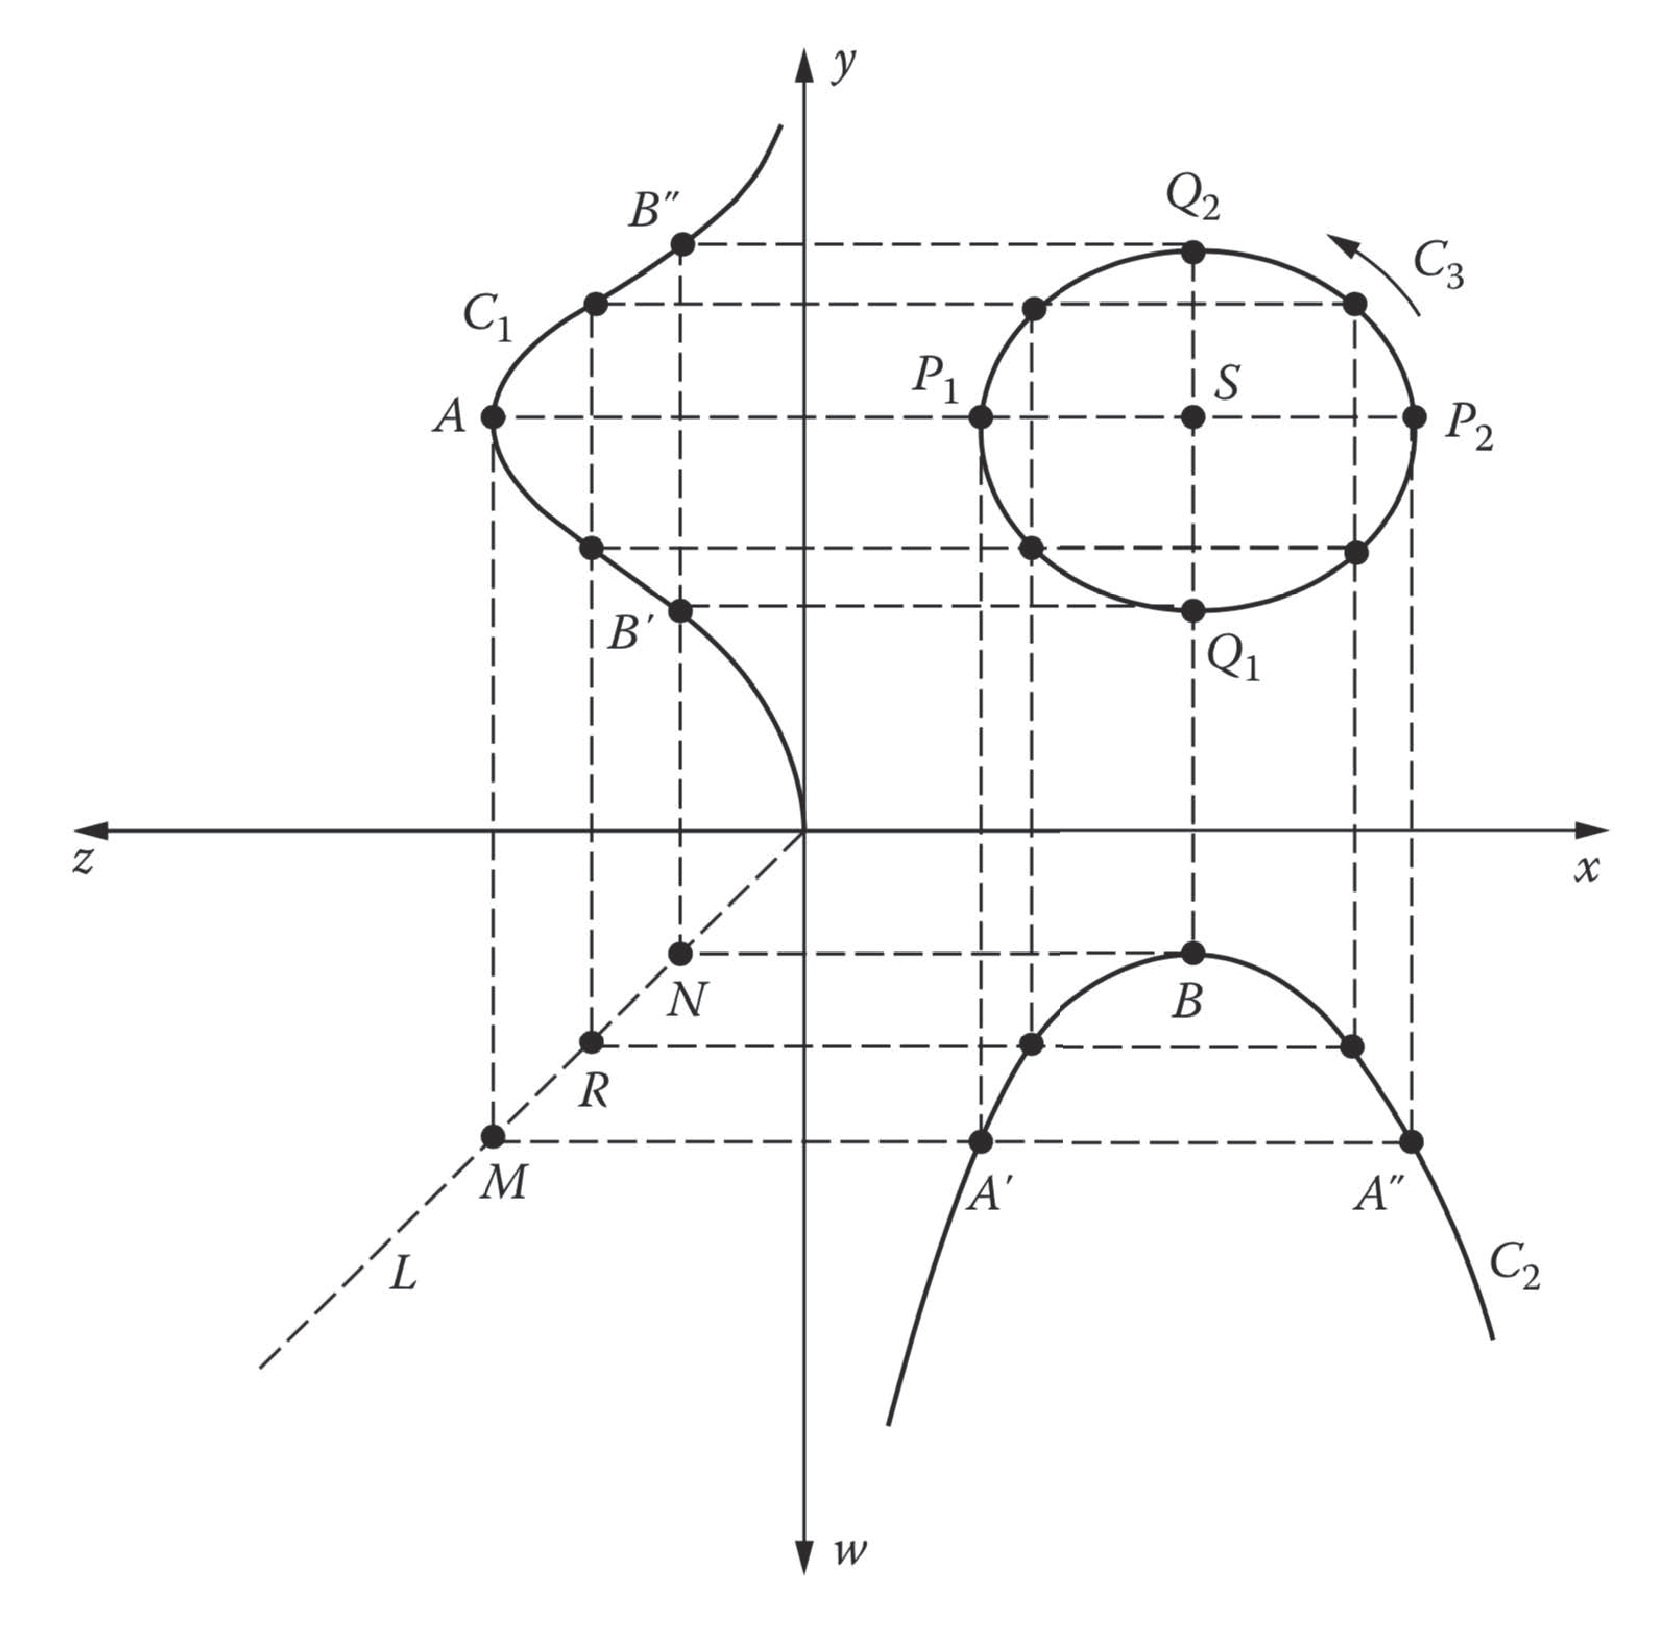
\includegraphics[height=8.cm, angle=0]{Volterra.eps}
\label{fig:Volterra}
\end{figure}
\vfill
%*************************************************************************









%%%%%%%%%%%%%%%%%%%%%%%%%%%%%%%%%%%%%%%%%%%%%%%%%%%%%%%%%%%%%%%%%%%%%%
\bibliographystyle{unsrt_update}
\bibliography{ref}
%%%%%%%%%%%%%%%%%%%%%%%%%%%%%%%%%%%%%%%%%%%%%%%%%%%%%%%%%%%%%%%%%%%%%%

\end{document}